% Options for packages loaded elsewhere
\PassOptionsToPackage{unicode}{hyperref}
\PassOptionsToPackage{hyphens}{url}
%
\documentclass[
  ignorenonframetext,
]{beamer}
\usepackage{pgfpages}
\setbeamertemplate{caption}[numbered]
\setbeamertemplate{caption label separator}{: }
\setbeamercolor{caption name}{fg=normal text.fg}
\beamertemplatenavigationsymbolsempty
% Prevent slide breaks in the middle of a paragraph
\widowpenalties 1 10000
\raggedbottom
\setbeamertemplate{part page}{
  \centering
  \begin{beamercolorbox}[sep=16pt,center]{part title}
    \usebeamerfont{part title}\insertpart\par
  \end{beamercolorbox}
}
\setbeamertemplate{section page}{
  \centering
  \begin{beamercolorbox}[sep=12pt,center]{part title}
    \usebeamerfont{section title}\insertsection\par
  \end{beamercolorbox}
}
\setbeamertemplate{subsection page}{
  \centering
  \begin{beamercolorbox}[sep=8pt,center]{part title}
    \usebeamerfont{subsection title}\insertsubsection\par
  \end{beamercolorbox}
}
\AtBeginPart{
  \frame{\partpage}
}
\AtBeginSection{
  \ifbibliography
  \else
    \frame{\sectionpage}
  \fi
}
\AtBeginSubsection{
  \frame{\subsectionpage}
}
\usepackage{amsmath,amssymb}
\usepackage{iftex}
\ifPDFTeX
  \usepackage[T1]{fontenc}
  \usepackage[utf8]{inputenc}
  \usepackage{textcomp} % provide euro and other symbols
\else % if luatex or xetex
  \usepackage{unicode-math} % this also loads fontspec
  \defaultfontfeatures{Scale=MatchLowercase}
  \defaultfontfeatures[\rmfamily]{Ligatures=TeX,Scale=1}
\fi
\usepackage{lmodern}
\usetheme[]{Madrid}
\ifPDFTeX\else
  % xetex/luatex font selection
\fi
% Use upquote if available, for straight quotes in verbatim environments
\IfFileExists{upquote.sty}{\usepackage{upquote}}{}
\IfFileExists{microtype.sty}{% use microtype if available
  \usepackage[]{microtype}
  \UseMicrotypeSet[protrusion]{basicmath} % disable protrusion for tt fonts
}{}
\makeatletter
\@ifundefined{KOMAClassName}{% if non-KOMA class
  \IfFileExists{parskip.sty}{%
    \usepackage{parskip}
  }{% else
    \setlength{\parindent}{0pt}
    \setlength{\parskip}{6pt plus 2pt minus 1pt}}
}{% if KOMA class
  \KOMAoptions{parskip=half}}
\makeatother
\usepackage{xcolor}
\newif\ifbibliography
\usepackage{color}
\usepackage{fancyvrb}
\newcommand{\VerbBar}{|}
\newcommand{\VERB}{\Verb[commandchars=\\\{\}]}
\DefineVerbatimEnvironment{Highlighting}{Verbatim}{commandchars=\\\{\}}
% Add ',fontsize=\small' for more characters per line
\usepackage{framed}
\definecolor{shadecolor}{RGB}{248,248,248}
\newenvironment{Shaded}{\begin{snugshade}}{\end{snugshade}}
\newcommand{\AlertTok}[1]{\textcolor[rgb]{0.94,0.16,0.16}{#1}}
\newcommand{\AnnotationTok}[1]{\textcolor[rgb]{0.56,0.35,0.01}{\textbf{\textit{#1}}}}
\newcommand{\AttributeTok}[1]{\textcolor[rgb]{0.13,0.29,0.53}{#1}}
\newcommand{\BaseNTok}[1]{\textcolor[rgb]{0.00,0.00,0.81}{#1}}
\newcommand{\BuiltInTok}[1]{#1}
\newcommand{\CharTok}[1]{\textcolor[rgb]{0.31,0.60,0.02}{#1}}
\newcommand{\CommentTok}[1]{\textcolor[rgb]{0.56,0.35,0.01}{\textit{#1}}}
\newcommand{\CommentVarTok}[1]{\textcolor[rgb]{0.56,0.35,0.01}{\textbf{\textit{#1}}}}
\newcommand{\ConstantTok}[1]{\textcolor[rgb]{0.56,0.35,0.01}{#1}}
\newcommand{\ControlFlowTok}[1]{\textcolor[rgb]{0.13,0.29,0.53}{\textbf{#1}}}
\newcommand{\DataTypeTok}[1]{\textcolor[rgb]{0.13,0.29,0.53}{#1}}
\newcommand{\DecValTok}[1]{\textcolor[rgb]{0.00,0.00,0.81}{#1}}
\newcommand{\DocumentationTok}[1]{\textcolor[rgb]{0.56,0.35,0.01}{\textbf{\textit{#1}}}}
\newcommand{\ErrorTok}[1]{\textcolor[rgb]{0.64,0.00,0.00}{\textbf{#1}}}
\newcommand{\ExtensionTok}[1]{#1}
\newcommand{\FloatTok}[1]{\textcolor[rgb]{0.00,0.00,0.81}{#1}}
\newcommand{\FunctionTok}[1]{\textcolor[rgb]{0.13,0.29,0.53}{\textbf{#1}}}
\newcommand{\ImportTok}[1]{#1}
\newcommand{\InformationTok}[1]{\textcolor[rgb]{0.56,0.35,0.01}{\textbf{\textit{#1}}}}
\newcommand{\KeywordTok}[1]{\textcolor[rgb]{0.13,0.29,0.53}{\textbf{#1}}}
\newcommand{\NormalTok}[1]{#1}
\newcommand{\OperatorTok}[1]{\textcolor[rgb]{0.81,0.36,0.00}{\textbf{#1}}}
\newcommand{\OtherTok}[1]{\textcolor[rgb]{0.56,0.35,0.01}{#1}}
\newcommand{\PreprocessorTok}[1]{\textcolor[rgb]{0.56,0.35,0.01}{\textit{#1}}}
\newcommand{\RegionMarkerTok}[1]{#1}
\newcommand{\SpecialCharTok}[1]{\textcolor[rgb]{0.81,0.36,0.00}{\textbf{#1}}}
\newcommand{\SpecialStringTok}[1]{\textcolor[rgb]{0.31,0.60,0.02}{#1}}
\newcommand{\StringTok}[1]{\textcolor[rgb]{0.31,0.60,0.02}{#1}}
\newcommand{\VariableTok}[1]{\textcolor[rgb]{0.00,0.00,0.00}{#1}}
\newcommand{\VerbatimStringTok}[1]{\textcolor[rgb]{0.31,0.60,0.02}{#1}}
\newcommand{\WarningTok}[1]{\textcolor[rgb]{0.56,0.35,0.01}{\textbf{\textit{#1}}}}
\usepackage{graphicx}
\makeatletter
\def\maxwidth{\ifdim\Gin@nat@width>\linewidth\linewidth\else\Gin@nat@width\fi}
\def\maxheight{\ifdim\Gin@nat@height>\textheight\textheight\else\Gin@nat@height\fi}
\makeatother
% Scale images if necessary, so that they will not overflow the page
% margins by default, and it is still possible to overwrite the defaults
% using explicit options in \includegraphics[width, height, ...]{}
\setkeys{Gin}{width=\maxwidth,height=\maxheight,keepaspectratio}
% Set default figure placement to htbp
\makeatletter
\def\fps@figure{htbp}
\makeatother
\setlength{\emergencystretch}{3em} % prevent overfull lines
\providecommand{\tightlist}{%
  \setlength{\itemsep}{0pt}\setlength{\parskip}{0pt}}
\setcounter{secnumdepth}{-\maxdimen} % remove section numbering
\logo{
\includegraphics[height=1cm,width=3cm]{logo.png}}
\usetheme{Madrid}
\usefonttheme{serif}
\setbeamertemplate{navigation symbols}{}
\usepackage{lmodern}  % for bold teletype font
\usepackage{amsmath}  % for \hookrightarrow
\usepackage{xcolor}   % for \textcolor


\ifLuaTeX
  \usepackage{selnolig}  % disable illegal ligatures
\fi
\usepackage{bookmark}
\IfFileExists{xurl.sty}{\usepackage{xurl}}{} % add URL line breaks if available
\urlstyle{same}
\hypersetup{
  pdftitle={Leksioni 14},
  pdfauthor={Endri Raco},
  hidelinks,
  pdfcreator={LaTeX via pandoc}}

\title{Leksioni 14}
\author{Endri Raco}
\date{21 July, 2024}

\begin{document}
\frame{\titlepage}

\begin{frame}[allowframebreaks]
  \tableofcontents[hideallsubsections]
\end{frame}
\section{}\label{section}

\begin{frame}[fragile]{Funksioni SQL AVG()}
\phantomsection\label{funksioni-sql-avg}
\begin{itemize}
\tightlist
\item
  Funksioni \texttt{AVG()} kthen vlerën mesatare të një kolone numerike.
\end{itemize}
\end{frame}

\begin{frame}[fragile]{Funksioni SQL AVG()}
\phantomsection\label{funksioni-sql-avg-1}
\begin{itemize}
\tightlist
\item
  Sintaksa:
\end{itemize}

\begin{Shaded}
\begin{Highlighting}[]
\KeywordTok{SELECT} \FunctionTok{AVG}\NormalTok{(kolona\_emri)}
\KeywordTok{FROM}\NormalTok{ tabela\_emri}
\KeywordTok{WHERE}\NormalTok{ kushti;}
\end{Highlighting}
\end{Shaded}
\end{frame}

\begin{frame}[fragile]{Shembull: Mesatarja e Çmimit të Produkteve}
\phantomsection\label{shembull-mesatarja-e-uxe7mimit-tuxeb-produkteve}
\AddToHookNext{env/Highlighting/begin}{\tiny}

\begin{Shaded}
\begin{Highlighting}[]
\NormalTok{\#\# Tabela e produkteve që do të përdorim }

\CommentTok{{-}{-} Krijo tabelën Products}
\KeywordTok{CREATE} \KeywordTok{TABLE}\NormalTok{ Products (}
\NormalTok{    ProductID }\DataTypeTok{int}\NormalTok{,}
\NormalTok{    ProductName }\DataTypeTok{varchar}\NormalTok{(}\DecValTok{255}\NormalTok{),}
\NormalTok{    SupplierID }\DataTypeTok{int}\NormalTok{,}
\NormalTok{    CategoryID }\DataTypeTok{int}\NormalTok{,}
\NormalTok{    Unit }\DataTypeTok{varchar}\NormalTok{(}\DecValTok{255}\NormalTok{),}
\NormalTok{    Price }\DataTypeTok{float}
\NormalTok{);}
\end{Highlighting}
\end{Shaded}
\end{frame}

\begin{frame}[fragile]{Shembull: Mesatarja e Çmimit të Produkteve}
\phantomsection\label{shembull-mesatarja-e-uxe7mimit-tuxeb-produkteve-1}
\AddToHookNext{env/Highlighting/begin}{\tiny}

\begin{Shaded}
\begin{Highlighting}[]
\CommentTok{{-}{-} Shto të dhënat në tabelën Products}
\KeywordTok{INSERT} \KeywordTok{INTO}\NormalTok{ Products (ProductID, ProductName, SupplierID, CategoryID, Unit, Price) }\KeywordTok{VALUES}
\NormalTok{(}\DecValTok{1}\NormalTok{, }\StringTok{\textquotesingle{}Chais\textquotesingle{}}\NormalTok{, }\DecValTok{1}\NormalTok{, }\DecValTok{1}\NormalTok{, }\StringTok{\textquotesingle{}10 boxes x 20 bags\textquotesingle{}}\NormalTok{, }\DecValTok{18}\NormalTok{),}
\NormalTok{(}\DecValTok{2}\NormalTok{, }\StringTok{\textquotesingle{}Chang\textquotesingle{}}\NormalTok{, }\DecValTok{1}\NormalTok{, }\DecValTok{1}\NormalTok{, }\StringTok{\textquotesingle{}24 {-} 12 oz bottles\textquotesingle{}}\NormalTok{, }\DecValTok{19}\NormalTok{),}
\NormalTok{(}\DecValTok{3}\NormalTok{, }\StringTok{\textquotesingle{}Aniseed Syrup\textquotesingle{}}\NormalTok{, }\DecValTok{1}\NormalTok{, }\DecValTok{2}\NormalTok{, }\StringTok{\textquotesingle{}12 {-} 550 ml bottles\textquotesingle{}}\NormalTok{, }\DecValTok{10}\NormalTok{),}
\NormalTok{(}\DecValTok{4}\NormalTok{, }\StringTok{\textquotesingle{}Chef Anton}\CharTok{\textquotesingle{}\textquotesingle{}}\StringTok{s Cajun Seasoning\textquotesingle{}}\NormalTok{, }\DecValTok{2}\NormalTok{, }\DecValTok{2}\NormalTok{, }\StringTok{\textquotesingle{}48 {-} 6 oz jars\textquotesingle{}}\NormalTok{, }\DecValTok{22}\NormalTok{),}
\NormalTok{(}\DecValTok{5}\NormalTok{, }\StringTok{\textquotesingle{}Chef Anton}\CharTok{\textquotesingle{}\textquotesingle{}}\StringTok{s Gumbo Mix\textquotesingle{}}\NormalTok{, }\DecValTok{2}\NormalTok{, }\DecValTok{2}\NormalTok{, }\StringTok{\textquotesingle{}36 boxes\textquotesingle{}}\NormalTok{, }\FloatTok{21.35}\NormalTok{);}
\end{Highlighting}
\end{Shaded}
\end{frame}

\begin{frame}[fragile]{Shtimi i Klauzolës WHERE}
\phantomsection\label{shtimi-i-klauzoluxebs-where}
Shembull: Mesatarja e çmimit të produkteve në kategorinë 1:

\AddToHookNext{env/Highlighting/begin}{\tiny}

\begin{Shaded}
\begin{Highlighting}[]
\KeywordTok{SELECT} \FunctionTok{AVG}\NormalTok{(Price)}
\KeywordTok{FROM}\NormalTok{ Products}
\KeywordTok{WHERE}\NormalTok{ CategoryID }\OperatorTok{=} \DecValTok{1}\NormalTok{;}
\end{Highlighting}
\end{Shaded}
\end{frame}

\begin{frame}{Shembull}
\phantomsection\label{shembull}
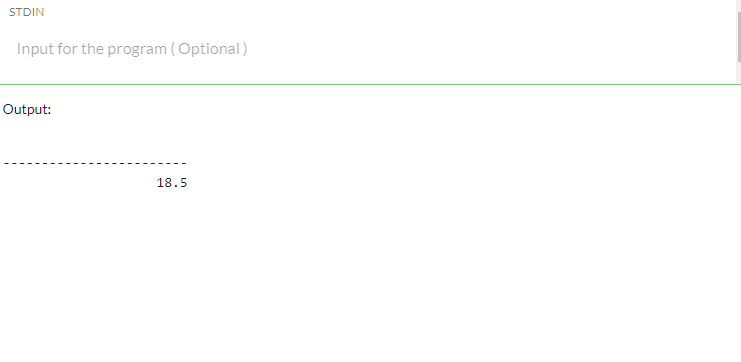
\includegraphics{./Figs/query57.png}
\end{frame}

\begin{frame}[fragile]{Përdorimi i Alias-it}
\phantomsection\label{puxebrdorimi-i-alias-it}
Shembull: Emërtimi i kolonës mesatare të çmimit si ``çmimi mesatar'':

\AddToHookNext{env/Highlighting/begin}{\tiny}

\begin{Shaded}
\begin{Highlighting}[]

\KeywordTok{SELECT} \FunctionTok{AVG}\NormalTok{(Price) }\KeywordTok{AS}\NormalTok{ [çmimi mesatar]}
\KeywordTok{FROM}\NormalTok{ Products;}
\end{Highlighting}
\end{Shaded}
\end{frame}

\begin{frame}{Shembull}
\phantomsection\label{shembull-1}
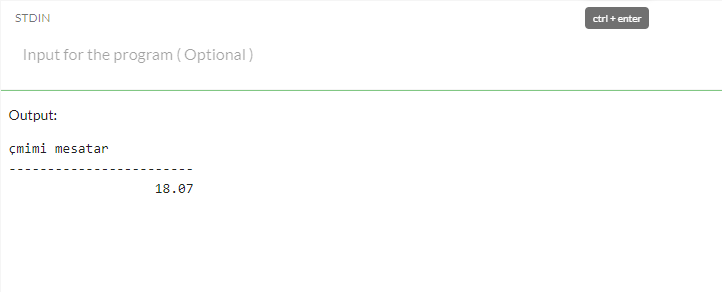
\includegraphics{./Figs/query58.png}
\end{frame}

\begin{frame}[fragile]{Produkte me Çmim Më të Lartë se Mesatarja}
\phantomsection\label{produkte-me-uxe7mim-muxeb-tuxeb-lartuxeb-se-mesatarja}
Shembull: Të gjitha produktet me çmim më të lartë se mesatarja:

\AddToHookNext{env/Highlighting/begin}{\tiny}

\begin{Shaded}
\begin{Highlighting}[]
\KeywordTok{SELECT} \OperatorTok{*}
\KeywordTok{FROM}\NormalTok{ Products}
\KeywordTok{WHERE}\NormalTok{ Price }\OperatorTok{\textgreater{}}\NormalTok{ (}\KeywordTok{SELECT} \FunctionTok{AVG}\NormalTok{(Price) }\KeywordTok{FROM}\NormalTok{ Products);}
\end{Highlighting}
\end{Shaded}
\end{frame}

\begin{frame}{Shembull}
\phantomsection\label{shembull-2}
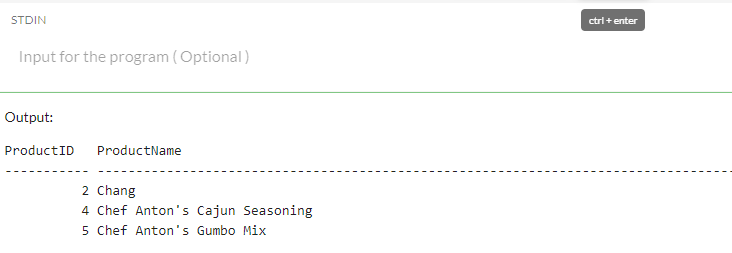
\includegraphics{./Figs/query59.png}
\end{frame}

\begin{frame}[fragile]{Përdorimi i AVG() me GROUP BY}
\phantomsection\label{puxebrdorimi-i-avg-me-group-by}
Shembull: Mesatarja e çmimit për çdo kategori në tabelën e Produkteve:

\AddToHookNext{env/Highlighting/begin}{\tiny}

\begin{Shaded}
\begin{Highlighting}[]
\KeywordTok{SELECT} \FunctionTok{AVG}\NormalTok{(Price) }\KeywordTok{AS}\NormalTok{ MesatarjaECmimit, CategoryID}
\KeywordTok{FROM}\NormalTok{ Products}
\KeywordTok{GROUP} \KeywordTok{BY}\NormalTok{ CategoryID;}
\end{Highlighting}
\end{Shaded}
\end{frame}

\begin{frame}{Shembull}
\phantomsection\label{shembull-3}
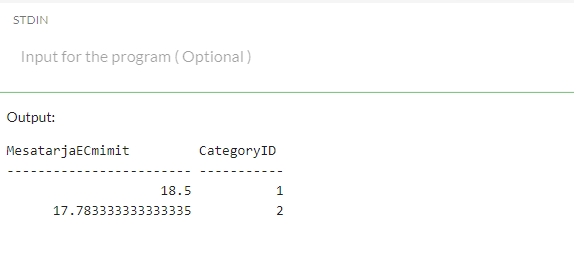
\includegraphics{./Figs/query60.png}
\end{frame}

\begin{frame}[fragile]{Funksioni SQL LIKE}
\phantomsection\label{funksioni-sql-like}
Operatori LIKE përdoret në klauzolën \textbf{WHERE} për të kërkuar një
model të specifikuar në një kolonë.

\AddToHookNext{env/Highlighting/begin}{\tiny}

\begin{Shaded}
\begin{Highlighting}[]
\KeywordTok{SELECT}\NormalTok{ kolona1, kolona2, }\OperatorTok{..}\NormalTok{.}
\KeywordTok{FROM}\NormalTok{ tabela\_emri}
\KeywordTok{WHERE}\NormalTok{ kolonaN }\KeywordTok{LIKE}\NormalTok{ modeli;}
\end{Highlighting}
\end{Shaded}
\end{frame}

\begin{frame}[fragile]{Tabela e klientëve që do të përdorim për
shembujt}
\phantomsection\label{tabela-e-klientuxebve-quxeb-do-tuxeb-puxebrdorim-puxebr-shembujt}
\AddToHookNext{env/Highlighting/begin}{\tiny}

\begin{Shaded}
\begin{Highlighting}[]
\CommentTok{{-}{-} Krijo tabelën Customers}
\KeywordTok{CREATE} \KeywordTok{TABLE}\NormalTok{ Customers (}
\NormalTok{    CustomerID }\DataTypeTok{int}\NormalTok{,}
\NormalTok{    CustomerName }\DataTypeTok{varchar}\NormalTok{(}\DecValTok{255}\NormalTok{),}
\NormalTok{    ContactName }\DataTypeTok{varchar}\NormalTok{(}\DecValTok{255}\NormalTok{),}
\NormalTok{    Address }\DataTypeTok{varchar}\NormalTok{(}\DecValTok{255}\NormalTok{),}
\NormalTok{    City }\DataTypeTok{varchar}\NormalTok{(}\DecValTok{255}\NormalTok{),}
\NormalTok{    PostalCode }\DataTypeTok{varchar}\NormalTok{(}\DecValTok{50}\NormalTok{),}
\NormalTok{    Country }\DataTypeTok{varchar}\NormalTok{(}\DecValTok{100}\NormalTok{)}
\NormalTok{);}
\end{Highlighting}
\end{Shaded}
\end{frame}

\begin{frame}[fragile]{Tabela e klientëve që do të përdorim për
shembujt}
\phantomsection\label{tabela-e-klientuxebve-quxeb-do-tuxeb-puxebrdorim-puxebr-shembujt-1}
\AddToHookNext{env/Highlighting/begin}{\tiny}

\begin{Shaded}
\begin{Highlighting}[]
\CommentTok{{-}{-} Shto të dhënat në tabelën Customers}
\KeywordTok{INSERT} \KeywordTok{INTO}\NormalTok{ Customers (CustomerID, CustomerName, ContactName, Address, City, PostalCode, Country) }\KeywordTok{VALUES}
\NormalTok{(}\DecValTok{1}\NormalTok{, }\StringTok{\textquotesingle{}Alfreds Futterkiste\textquotesingle{}}\NormalTok{, }\StringTok{\textquotesingle{}Maria Anders\textquotesingle{}}\NormalTok{, }\StringTok{\textquotesingle{}Obere Str. 57\textquotesingle{}}\NormalTok{, }\StringTok{\textquotesingle{}Berlin\textquotesingle{}}\NormalTok{, }\StringTok{\textquotesingle{}12209\textquotesingle{}}\NormalTok{, }\StringTok{\textquotesingle{}Germany\textquotesingle{}}\NormalTok{),}
\NormalTok{(}\DecValTok{2}\NormalTok{, }\StringTok{\textquotesingle{}Ana Trujillo Emparedados y helados\textquotesingle{}}\NormalTok{, }\StringTok{\textquotesingle{}Ana Trujillo\textquotesingle{}}\NormalTok{, }\StringTok{\textquotesingle{}Avda. de la Constitución 2222\textquotesingle{}}\NormalTok{, }\StringTok{\textquotesingle{}México D.F.\textquotesingle{}}\NormalTok{, }\StringTok{\textquotesingle{}05021\textquotesingle{}}\NormalTok{, }\StringTok{\textquotesingle{}Mexico\textquotesingle{}}\NormalTok{),}
\NormalTok{(}\DecValTok{3}\NormalTok{, }\StringTok{\textquotesingle{}Antonio Moreno Taquería\textquotesingle{}}\NormalTok{, }\StringTok{\textquotesingle{}Antonio Moreno\textquotesingle{}}\NormalTok{, }\StringTok{\textquotesingle{}Mataderos 2312\textquotesingle{}}\NormalTok{, }\StringTok{\textquotesingle{}México D.F.\textquotesingle{}}\NormalTok{, }\StringTok{\textquotesingle{}05023\textquotesingle{}}\NormalTok{, }\StringTok{\textquotesingle{}Mexico\textquotesingle{}}\NormalTok{),}
\NormalTok{(}\DecValTok{4}\NormalTok{, }\StringTok{\textquotesingle{}Around the Horn\textquotesingle{}}\NormalTok{, }\StringTok{\textquotesingle{}Thomas Hardy\textquotesingle{}}\NormalTok{, }\StringTok{\textquotesingle{}120 Hanover Sq.\textquotesingle{}}\NormalTok{, }\StringTok{\textquotesingle{}London\textquotesingle{}}\NormalTok{, }\StringTok{\textquotesingle{}WA1 1DP\textquotesingle{}}\NormalTok{, }\StringTok{\textquotesingle{}UK\textquotesingle{}}\NormalTok{),}
\NormalTok{(}\DecValTok{5}\NormalTok{, }\StringTok{\textquotesingle{}Berglunds snabbköp\textquotesingle{}}\NormalTok{, }\StringTok{\textquotesingle{}Christina Berglund\textquotesingle{}}\NormalTok{, }\StringTok{\textquotesingle{}Berguvsvägen 8\textquotesingle{}}\NormalTok{, }\StringTok{\textquotesingle{}Luleå\textquotesingle{}}\NormalTok{, }\StringTok{\textquotesingle{}S{-}958 22\textquotesingle{}}\NormalTok{, }\StringTok{\textquotesingle{}Sweden\textquotesingle{}}\NormalTok{);}
\end{Highlighting}
\end{Shaded}
\end{frame}

\begin{frame}[fragile]{Fillon me një shkronjë të caktuar}
\phantomsection\label{fillon-me-njuxeb-shkronjuxeb-tuxeb-caktuar}
\begin{Shaded}
\begin{Highlighting}[]
\KeywordTok{SELECT} \OperatorTok{*}
\KeywordTok{FROM}\NormalTok{ Customers}
\KeywordTok{WHERE}\NormalTok{ CustomerName }\KeywordTok{LIKE} \StringTok{\textquotesingle{}a\%\textquotesingle{}}\NormalTok{;}
\end{Highlighting}
\end{Shaded}
\end{frame}

\begin{frame}{Shembull}
\phantomsection\label{shembull-4}
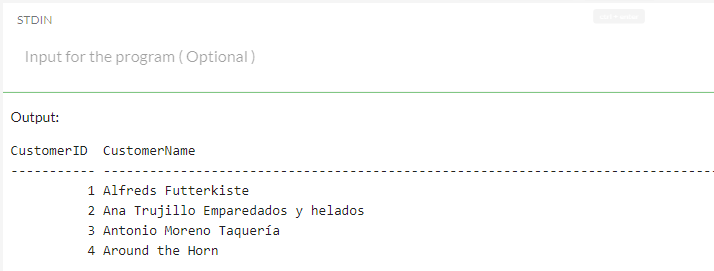
\includegraphics{./Figs/query61.png}
\end{frame}

\begin{frame}{Wildcard}
\phantomsection\label{wildcard}
\begin{itemize}
\item
  Wildcard \(\_\) përfaqëson një karakter të vetëm.
\item
  Shembull: Qyteti që fillon me `L' dhe përfundon me dy wildcard
  karaktere
\end{itemize}
\end{frame}

\begin{frame}[fragile]{Wildcard}
\phantomsection\label{wildcard-1}
\begin{Shaded}
\begin{Highlighting}[]
\KeywordTok{SELECT} \OperatorTok{*}
\KeywordTok{FROM}\NormalTok{ Customers}
\KeywordTok{WHERE}\NormalTok{ City }\KeywordTok{LIKE} \StringTok{\textquotesingle{}L\_nd\_\_\textquotesingle{}}\NormalTok{;}
\end{Highlighting}
\end{Shaded}
\end{frame}

\begin{frame}{Shembull}
\phantomsection\label{shembull-5}
\begin{itemize}
\item
  The \(%
  \) Wildcard
\item
  Wildcard \(%
  \) përfaqëson çdo numër karakteresh, përfshirë zero karaktere.
\item
  Shembull: Qyteti që përmban shkronjën `L'
\end{itemize}
\end{frame}

\begin{frame}[fragile]{Wildcard}
\phantomsection\label{wildcard-2}
\begin{Shaded}
\begin{Highlighting}[]
\KeywordTok{SELECT} \OperatorTok{*}
\KeywordTok{FROM}\NormalTok{ Customers}
\KeywordTok{WHERE}\NormalTok{ City }\KeywordTok{LIKE} \StringTok{\textquotesingle{}\%L\%\textquotesingle{}}\NormalTok{;}
\end{Highlighting}
\end{Shaded}
\end{frame}

\begin{frame}{Shembull}
\phantomsection\label{shembull-6}
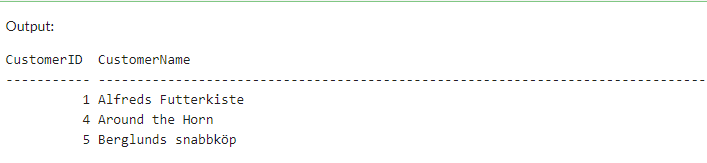
\includegraphics{./Figs/query62.png}
\end{frame}

\begin{frame}{Fillon me}
\phantomsection\label{fillon-me}
Për të kthyer të dhëna që fillojnë me një shkronjë ose frazë specifike,
shtoni \(%
\) në fund të shkronjës ose frazës.
\end{frame}

\begin{frame}[fragile]{Shembull: Fillon me `Al'}
\phantomsection\label{shembull-fillon-me-al}
\AddToHookNext{env/Highlighting/begin}{\tiny}

\begin{Shaded}
\begin{Highlighting}[]
\KeywordTok{SELECT} \OperatorTok{*}
\KeywordTok{FROM}\NormalTok{ Customers}
\KeywordTok{WHERE}\NormalTok{ CustomerName }\KeywordTok{LIKE} \StringTok{\textquotesingle{}Al\%\textquotesingle{}}\NormalTok{;}
\end{Highlighting}
\end{Shaded}
\end{frame}

\begin{frame}{Shembull}
\phantomsection\label{shembull-7}
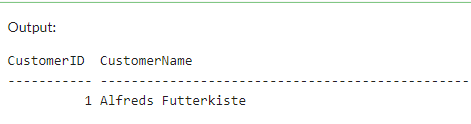
\includegraphics{./Figs/query63.png}
\end{frame}

\begin{frame}{Përfundon me}
\phantomsection\label{puxebrfundon-me}
Për të kthyer të dhëna që përfundojnë me një shkronjë ose frazë
specifike, shtoni \(%
\) në fillim të shkronjës ose frazës.
\end{frame}

\begin{frame}[fragile]{Shembull: Përfundon me `a'}
\phantomsection\label{shembull-puxebrfundon-me-a}
\begin{Shaded}
\begin{Highlighting}[]
\KeywordTok{SELECT} \OperatorTok{*}
\KeywordTok{FROM}\NormalTok{ Customers}
\KeywordTok{WHERE}\NormalTok{ CustomerName }\KeywordTok{LIKE} \StringTok{\textquotesingle{}\%a\textquotesingle{}}\NormalTok{;}
\end{Highlighting}
\end{Shaded}
\end{frame}

\begin{frame}{Shembull}
\phantomsection\label{shembull-8}
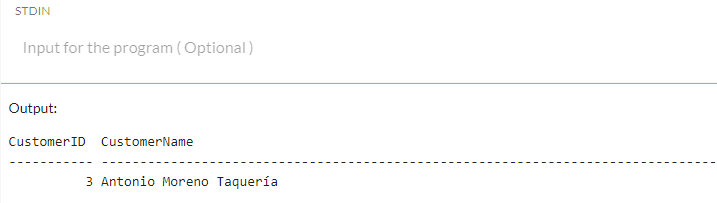
\includegraphics{./Figs/query64.png}
\end{frame}

\begin{frame}[fragile]{Përmban}
\phantomsection\label{puxebrmban}
\begin{itemize}
\tightlist
\item
  Për të kthyer të dhëna që përmbajnë një shkronjë ose frazë specifike,
  shtoni \(%
  \) para dhe pas shkronjës ose frazës. \#\# Shembull: Përmban frazën
  `or'
\end{itemize}

\begin{Shaded}
\begin{Highlighting}[]
\KeywordTok{SELECT} \OperatorTok{*}
\KeywordTok{FROM}\NormalTok{ Customers}
\KeywordTok{WHERE}\NormalTok{ CustomerName }\KeywordTok{LIKE} \StringTok{\textquotesingle{}\%or\%\textquotesingle{}}\NormalTok{;}
\end{Highlighting}
\end{Shaded}
\end{frame}

\begin{frame}{Shembull}
\phantomsection\label{shembull-9}
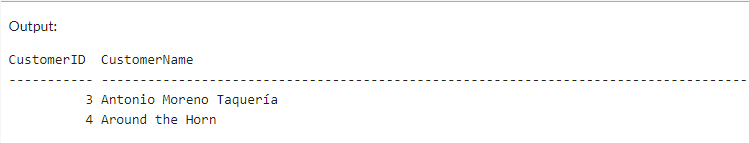
\includegraphics{./Figs/query65.png} \#\# Kombinimi i Wildcards

\begin{itemize}
\tightlist
\item
  Çdo wildcard, si \(%
  \) dhe \(\_\), mund të përdoret në kombinim me wildcard të tjerë.
\end{itemize}
\end{frame}

\begin{frame}[fragile]{Shembull: Fillon me `a' dhe ka të paktën 3
karaktere}
\phantomsection\label{shembull-fillon-me-a-dhe-ka-tuxeb-paktuxebn-3-karaktere}
\begin{Shaded}
\begin{Highlighting}[]
\KeywordTok{SELECT} \OperatorTok{*}
\KeywordTok{FROM}\NormalTok{ Customers}
\KeywordTok{WHERE}\NormalTok{ CustomerName }\KeywordTok{LIKE} \StringTok{\textquotesingle{}a\_\_\%\textquotesingle{}}\NormalTok{;}
\end{Highlighting}
\end{Shaded}
\end{frame}

\begin{frame}{Shembull}
\phantomsection\label{shembull-10}
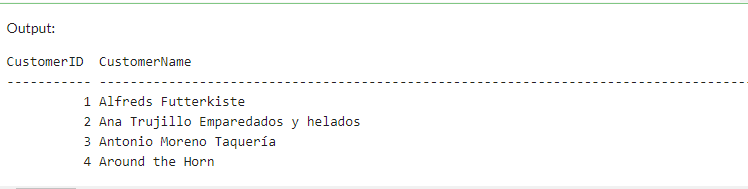
\includegraphics{./Figs/query66.png}
\end{frame}

\begin{frame}{Pa Wildcard}
\phantomsection\label{pa-wildcard}
\begin{itemize}
\tightlist
\item
  Nëse nuk specifikohet asnjë wildcard, fraza duhet të ketë një
  përputhje të saktë për të kthyer një rezultat.
\end{itemize}
\end{frame}

\begin{frame}[fragile]{Shembull: Nga Spanja}
\phantomsection\label{shembull-nga-spanja}
\begin{Shaded}
\begin{Highlighting}[]
\KeywordTok{SELECT} \OperatorTok{*}
\KeywordTok{FROM}\NormalTok{ Customers}
\KeywordTok{WHERE}\NormalTok{ Country }\KeywordTok{LIKE} \StringTok{\textquotesingle{}Spain\textquotesingle{}}\NormalTok{;}
\end{Highlighting}
\end{Shaded}
\end{frame}

\begin{frame}{Karakteret Wildcard në SQL}
\phantomsection\label{karakteret-wildcard-nuxeb-sql}
\begin{itemize}
\item
  Një karakter wildcard përdoret për të zëvendësuar një ose më shumë
  karaktere në një varg.
\item
  Karakteret wildcard përdoren me operatorin LIKE.
\item
  Operatori LIKE përdoret në klauzolën WHERE për të kërkuar një model të
  specifikuar në një kolonë.
\end{itemize}
\end{frame}

\begin{frame}[fragile]{Sintaksa}
\phantomsection\label{sintaksa}
\begin{Shaded}
\begin{Highlighting}[]
\KeywordTok{SELECT}\NormalTok{ kolona1, kolona2, }\OperatorTok{..}\NormalTok{.}
\KeywordTok{FROM}\NormalTok{ tabela\_emri}
\KeywordTok{WHERE}\NormalTok{ kolonaN }\KeywordTok{LIKE}\NormalTok{ modeli;}
\end{Highlighting}
\end{Shaded}
\end{frame}

\begin{frame}[fragile]{SQL Query për Krijimin e Tabelës ``Customers''
dhe Shtimin e Të Dhënave}
\phantomsection\label{sql-query-puxebr-krijimin-e-tabeluxebs-customers-dhe-shtimin-e-tuxeb-dhuxebnave}
\AddToHookNext{env/Highlighting/begin}{\tiny}

\begin{Shaded}
\begin{Highlighting}[]
\CommentTok{{-}{-} Krijo tabelën Customers}
\KeywordTok{CREATE} \KeywordTok{TABLE}\NormalTok{ Customers (}
\NormalTok{    CustomerID }\DataTypeTok{int}\NormalTok{,}
\NormalTok{    CustomerName }\DataTypeTok{varchar}\NormalTok{(}\DecValTok{255}\NormalTok{),}
\NormalTok{    ContactName }\DataTypeTok{varchar}\NormalTok{(}\DecValTok{255}\NormalTok{),}
\NormalTok{    Address }\DataTypeTok{varchar}\NormalTok{(}\DecValTok{255}\NormalTok{),}
\NormalTok{    City }\DataTypeTok{varchar}\NormalTok{(}\DecValTok{255}\NormalTok{),}
\NormalTok{    PostalCode }\DataTypeTok{varchar}\NormalTok{(}\DecValTok{50}\NormalTok{),}
\NormalTok{    Country }\DataTypeTok{varchar}\NormalTok{(}\DecValTok{100}\NormalTok{)}
\NormalTok{);}
\end{Highlighting}
\end{Shaded}
\end{frame}

\begin{frame}[fragile]{SQL Query për Krijimin e Tabelës ``Customers''
dhe Shtimin e Të Dhënave}
\phantomsection\label{sql-query-puxebr-krijimin-e-tabeluxebs-customers-dhe-shtimin-e-tuxeb-dhuxebnave-1}
\AddToHookNext{env/Highlighting/begin}{\tiny}

\begin{Shaded}
\begin{Highlighting}[]
\CommentTok{{-}{-} Shto të dhënat në tabelën Customers}
\KeywordTok{INSERT} \KeywordTok{INTO}\NormalTok{ Customers (CustomerID, CustomerName, ContactName, Address, City, PostalCode, Country) }\KeywordTok{VALUES}
\NormalTok{(}\DecValTok{1}\NormalTok{, }\StringTok{\textquotesingle{}Alfreds Futterkiste\textquotesingle{}}\NormalTok{, }\StringTok{\textquotesingle{}Maria Anders\textquotesingle{}}\NormalTok{, }\StringTok{\textquotesingle{}Obere Str. 57\textquotesingle{}}\NormalTok{, }\StringTok{\textquotesingle{}Berlin\textquotesingle{}}\NormalTok{, }\StringTok{\textquotesingle{}12209\textquotesingle{}}\NormalTok{, }\StringTok{\textquotesingle{}Germany\textquotesingle{}}\NormalTok{),}
\NormalTok{(}\DecValTok{2}\NormalTok{, }\StringTok{\textquotesingle{}Ana Trujillo Emparedados y helados\textquotesingle{}}\NormalTok{, }\StringTok{\textquotesingle{}Ana Trujillo\textquotesingle{}}\NormalTok{, }\StringTok{\textquotesingle{}Avda. de la Constitución 2222\textquotesingle{}}\NormalTok{, }\StringTok{\textquotesingle{}México D.F.\textquotesingle{}}\NormalTok{, }\StringTok{\textquotesingle{}05021\textquotesingle{}}\NormalTok{, }\StringTok{\textquotesingle{}Mexico\textquotesingle{}}\NormalTok{),}
\NormalTok{(}\DecValTok{3}\NormalTok{, }\StringTok{\textquotesingle{}Antonio Moreno Taquería\textquotesingle{}}\NormalTok{, }\StringTok{\textquotesingle{}Antonio Moreno\textquotesingle{}}\NormalTok{, }\StringTok{\textquotesingle{}Mataderos 2312\textquotesingle{}}\NormalTok{, }\StringTok{\textquotesingle{}México D.F.\textquotesingle{}}\NormalTok{, }\StringTok{\textquotesingle{}05023\textquotesingle{}}\NormalTok{, }\StringTok{\textquotesingle{}Mexico\textquotesingle{}}\NormalTok{),}
\NormalTok{(}\DecValTok{4}\NormalTok{, }\StringTok{\textquotesingle{}Around the Horn\textquotesingle{}}\NormalTok{, }\StringTok{\textquotesingle{}Thomas Hardy\textquotesingle{}}\NormalTok{, }\StringTok{\textquotesingle{}120 Hanover Sq.\textquotesingle{}}\NormalTok{, }\StringTok{\textquotesingle{}London\textquotesingle{}}\NormalTok{, }\StringTok{\textquotesingle{}WA1 1DP\textquotesingle{}}\NormalTok{, }\StringTok{\textquotesingle{}UK\textquotesingle{}}\NormalTok{),}
\NormalTok{(}\DecValTok{5}\NormalTok{, }\StringTok{\textquotesingle{}Berglunds snabbköp\textquotesingle{}}\NormalTok{, }\StringTok{\textquotesingle{}Christina Berglund\textquotesingle{}}\NormalTok{, }\StringTok{\textquotesingle{}Berguvsvägen 8\textquotesingle{}}\NormalTok{, }\StringTok{\textquotesingle{}Luleå\textquotesingle{}}\NormalTok{, }\StringTok{\textquotesingle{}S{-}958 22\textquotesingle{}}\NormalTok{, }\StringTok{\textquotesingle{}Sweden\textquotesingle{}}\NormalTok{);}
\end{Highlighting}
\end{Shaded}
\end{frame}

\begin{frame}{Përdorimi i Wildcard percentage}
\phantomsection\label{puxebrdorimi-i-wildcard-percentage}
\begin{itemize}
\tightlist
\item
  Wildcard \(%
  \) përfaqëson çdo numër karakteresh, përfshirë zero karaktere.
\end{itemize}
\end{frame}

\begin{frame}[fragile]{Shembull: Përfundon me `s'}
\phantomsection\label{shembull-puxebrfundon-me-s}
\begin{Shaded}
\begin{Highlighting}[]
\KeywordTok{SELECT} \OperatorTok{*}
\KeywordTok{FROM}\NormalTok{ Customers}
\KeywordTok{WHERE}\NormalTok{ CustomerName }\KeywordTok{LIKE} \StringTok{\textquotesingle{}\%s\textquotesingle{}}\NormalTok{;}
\end{Highlighting}
\end{Shaded}
\end{frame}

\begin{frame}{Shembull}
\phantomsection\label{shembull-11}
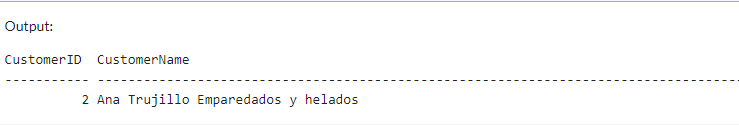
\includegraphics{./Figs/query67.png}
\end{frame}

\begin{frame}[fragile]{Shembull}
\phantomsection\label{shembull-12}
Shembull: Përmban `rou'

\begin{Shaded}
\begin{Highlighting}[]
\KeywordTok{SELECT} \OperatorTok{*}
\KeywordTok{FROM}\NormalTok{ Customers}
\KeywordTok{WHERE}\NormalTok{ CustomerName }\KeywordTok{LIKE} \StringTok{\textquotesingle{}\%rou\%\textquotesingle{}}\NormalTok{;}
\end{Highlighting}
\end{Shaded}
\end{frame}

\begin{frame}{Shembull}
\phantomsection\label{shembull-13}
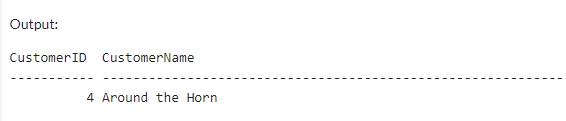
\includegraphics{./Figs/query68.png}
\end{frame}

\begin{frame}{Përdorimi i Wildcard \(\_\)}
\phantomsection\label{puxebrdorimi-i-wildcard-_}
Wildcard \(\_\) përfaqëson një karakter të vetëm.
\end{frame}

\begin{frame}[fragile]{Shembull: Qyteti që fillon me ndonjë karakter dhe
përfundon me `ondon'}
\phantomsection\label{shembull-qyteti-quxeb-fillon-me-ndonjuxeb-karakter-dhe-puxebrfundon-me-ondon}
\begin{Shaded}
\begin{Highlighting}[]
\KeywordTok{SELECT} \OperatorTok{*}
\KeywordTok{FROM}\NormalTok{ Customers}
\KeywordTok{WHERE}\NormalTok{ City }\KeywordTok{LIKE} \StringTok{\textquotesingle{}\_ondon\textquotesingle{}}\NormalTok{;}
\end{Highlighting}
\end{Shaded}
\end{frame}

\begin{frame}{Shembull}
\phantomsection\label{shembull-14}
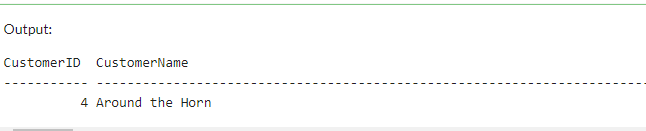
\includegraphics{./Figs/query69.png}
\end{frame}

\begin{frame}[fragile]{Shembull: Qyteti që fillon me `L', ndjekur nga 3
karaktere, përfundon me `on'}
\phantomsection\label{shembull-qyteti-quxeb-fillon-me-l-ndjekur-nga-3-karaktere-puxebrfundon-me-on}
\begin{Shaded}
\begin{Highlighting}[]
\KeywordTok{SELECT} \OperatorTok{*}
\KeywordTok{FROM}\NormalTok{ Customers}
\KeywordTok{WHERE}\NormalTok{ City }\KeywordTok{LIKE} \StringTok{\textquotesingle{}L\_\_\_on\textquotesingle{}}\NormalTok{;}
\end{Highlighting}
\end{Shaded}
\end{frame}

\begin{frame}{Shembull}
\phantomsection\label{shembull-15}
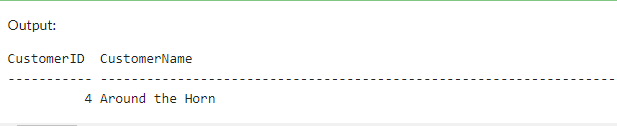
\includegraphics{./Figs/query70.png}
\end{frame}

\begin{frame}{Përdorimi i Wildcard {[}{]}}
\phantomsection\label{puxebrdorimi-i-wildcard}
\begin{itemize}
\tightlist
\item
  Wildcard {[}{]} kthen një rezultat nëse ndonjë nga karakteret brenda
  ka një përputhje.
\end{itemize}
\end{frame}

\begin{frame}[fragile]{Shembull: Fillon me `b', `s' ose `p'}
\phantomsection\label{shembull-fillon-me-b-s-ose-p}
\begin{Shaded}
\begin{Highlighting}[]
\KeywordTok{SELECT} \OperatorTok{*}
\KeywordTok{FROM}\NormalTok{ Customers}
\KeywordTok{WHERE}\NormalTok{ CustomerName }\KeywordTok{LIKE} \StringTok{\textquotesingle{}[bsp]\%\textquotesingle{}}\NormalTok{;}
\end{Highlighting}
\end{Shaded}
\end{frame}

\begin{frame}{Shembull}
\phantomsection\label{shembull-16}
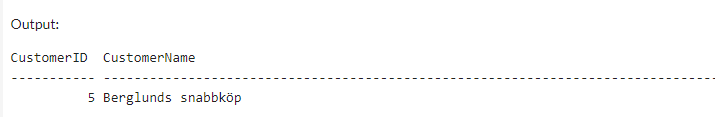
\includegraphics{./Figs/query71.png}
\end{frame}

\begin{frame}{Përdorimi i Wildcard -}
\phantomsection\label{puxebrdorimi-i-wildcard--}
\begin{itemize}
\tightlist
\item
  Wildcard - lejon specifikimin e një intervali karakteresh brenda
  wildcard {[}{]}.
\end{itemize}
\end{frame}

\begin{frame}[fragile]{Shembull: Fillon me `a', `b', `c', `d', `e' ose
`f'}
\phantomsection\label{shembull-fillon-me-a-b-c-d-e-ose-f}
\begin{Shaded}
\begin{Highlighting}[]
\KeywordTok{SELECT} \OperatorTok{*}
\KeywordTok{FROM}\NormalTok{ Customers}
\KeywordTok{WHERE}\NormalTok{ CustomerName }\KeywordTok{LIKE} \StringTok{\textquotesingle{}[a{-}f]\%\textquotesingle{}}\NormalTok{;}
\end{Highlighting}
\end{Shaded}
\end{frame}

\begin{frame}{Shembull}
\phantomsection\label{shembull-17}
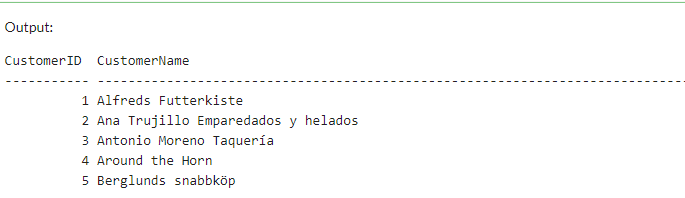
\includegraphics{./Figs/query72.png}
\end{frame}

\begin{frame}{Kombinimi i Wildcards}
\phantomsection\label{kombinimi-i-wildcards}
\begin{itemize}
\tightlist
\item
  Çdo wildcard, si \(%
  \) dhe \(\_\), mund të përdoret në kombinim me wildcard të tjerë.
\end{itemize}
\end{frame}

\begin{frame}[fragile]{Shembull: Fillon me `a' dhe ka të paktën 3
karaktere}
\phantomsection\label{shembull-fillon-me-a-dhe-ka-tuxeb-paktuxebn-3-karaktere-1}
\begin{Shaded}
\begin{Highlighting}[]
\KeywordTok{SELECT} \OperatorTok{*}
\KeywordTok{FROM}\NormalTok{ Customers}
\KeywordTok{WHERE}\NormalTok{ CustomerName }\KeywordTok{LIKE} \StringTok{\textquotesingle{}a\_\_\%\textquotesingle{}}\NormalTok{;}
\end{Highlighting}
\end{Shaded}
\end{frame}

\begin{frame}{Shembull}
\phantomsection\label{shembull-18}
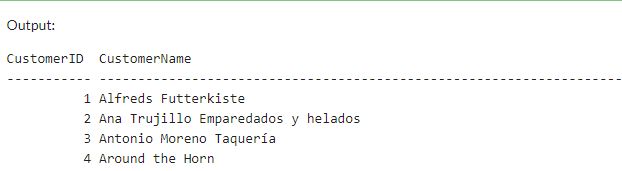
\includegraphics{./Figs/query73.png}
\end{frame}

\begin{frame}[fragile]{Shembull: Ka `r' në pozicionin e dytë}
\phantomsection\label{shembull-ka-r-nuxeb-pozicionin-e-dytuxeb}
\begin{Shaded}
\begin{Highlighting}[]
\KeywordTok{SELECT} \OperatorTok{*}
\KeywordTok{FROM}\NormalTok{ Customers}
\KeywordTok{WHERE}\NormalTok{ CustomerName }\KeywordTok{LIKE} \StringTok{\textquotesingle{}\_r\%\textquotesingle{}}\NormalTok{;}
\end{Highlighting}
\end{Shaded}
\end{frame}

\begin{frame}{Shembull}
\phantomsection\label{shembull-19}
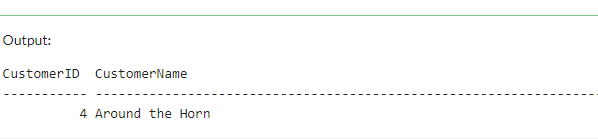
\includegraphics{./Figs/query74.png}
\end{frame}

\begin{frame}{Funksioni SQL IN}
\phantomsection\label{funksioni-sql-in}
\begin{itemize}
\item
  Operatori IN lejon specifikimin e vlerave të shumta në një klauzolë
  WHERE.
\item
  Operatori IN është një formë e shkurtër për kushtet e shumëfishta OR.
\end{itemize}
\end{frame}

\begin{frame}[fragile]{Sintaksa}
\phantomsection\label{sintaksa-1}
\AddToHookNext{env/Highlighting/begin}{\tiny}

\begin{Shaded}
\begin{Highlighting}[]
\KeywordTok{SELECT}\NormalTok{ kolona\_emri(a)}
\KeywordTok{FROM}\NormalTok{ tabela\_emri}
\KeywordTok{WHERE}\NormalTok{ kolona\_emri }\KeywordTok{IN}\NormalTok{ (vlera1, vlera2, }\OperatorTok{..}\NormalTok{.);}
\end{Highlighting}
\end{Shaded}
\end{frame}

\begin{frame}[fragile]{SQL Query për Krijimin e Tabelës ``Customers''
dhe Shtimin e Të Dhënave}
\phantomsection\label{sql-query-puxebr-krijimin-e-tabeluxebs-customers-dhe-shtimin-e-tuxeb-dhuxebnave-2}
\AddToHookNext{env/Highlighting/begin}{\tiny}

\begin{Shaded}
\begin{Highlighting}[]
\CommentTok{{-}{-} Krijo tabelën Customers}
\KeywordTok{CREATE} \KeywordTok{TABLE}\NormalTok{ Customers (}
\NormalTok{    CustomerID }\DataTypeTok{int}\NormalTok{,}
\NormalTok{    CustomerName }\DataTypeTok{varchar}\NormalTok{(}\DecValTok{255}\NormalTok{),}
\NormalTok{    ContactName }\DataTypeTok{varchar}\NormalTok{(}\DecValTok{255}\NormalTok{),}
\NormalTok{    Address }\DataTypeTok{varchar}\NormalTok{(}\DecValTok{255}\NormalTok{),}
\NormalTok{    City }\DataTypeTok{varchar}\NormalTok{(}\DecValTok{255}\NormalTok{),}
\NormalTok{    PostalCode }\DataTypeTok{varchar}\NormalTok{(}\DecValTok{50}\NormalTok{),}
\NormalTok{    Country }\DataTypeTok{varchar}\NormalTok{(}\DecValTok{100}\NormalTok{)}
\NormalTok{);}
\end{Highlighting}
\end{Shaded}
\end{frame}

\begin{frame}[fragile]{SQL Query për Krijimin e Tabelës ``Customers''
dhe Shtimin e Të Dhënave}
\phantomsection\label{sql-query-puxebr-krijimin-e-tabeluxebs-customers-dhe-shtimin-e-tuxeb-dhuxebnave-3}
\AddToHookNext{env/Highlighting/begin}{\tiny}

\begin{Shaded}
\begin{Highlighting}[]
\CommentTok{{-}{-} Shto të dhënat në tabelën Customers}
\KeywordTok{INSERT} \KeywordTok{INTO}\NormalTok{ Customers (CustomerID, CustomerName, ContactName, Address, City, PostalCode, Country) }\KeywordTok{VALUES}
\NormalTok{(}\DecValTok{1}\NormalTok{, }\StringTok{\textquotesingle{}Alfreds Futterkiste\textquotesingle{}}\NormalTok{, }\StringTok{\textquotesingle{}Maria Anders\textquotesingle{}}\NormalTok{, }\StringTok{\textquotesingle{}Obere Str. 57\textquotesingle{}}\NormalTok{, }\StringTok{\textquotesingle{}Berlin\textquotesingle{}}\NormalTok{, }\StringTok{\textquotesingle{}12209\textquotesingle{}}\NormalTok{, }\StringTok{\textquotesingle{}Germany\textquotesingle{}}\NormalTok{),}
\NormalTok{(}\DecValTok{2}\NormalTok{, }\StringTok{\textquotesingle{}Ana Trujillo Emparedados y helados\textquotesingle{}}\NormalTok{, }\StringTok{\textquotesingle{}Ana Trujillo\textquotesingle{}}\NormalTok{, }\StringTok{\textquotesingle{}Avda. de la Constitución 2222\textquotesingle{}}\NormalTok{, }\StringTok{\textquotesingle{}México D.F.\textquotesingle{}}\NormalTok{, }\StringTok{\textquotesingle{}05021\textquotesingle{}}\NormalTok{, }\StringTok{\textquotesingle{}Mexico\textquotesingle{}}\NormalTok{),}
\NormalTok{(}\DecValTok{3}\NormalTok{, }\StringTok{\textquotesingle{}Antonio Moreno Taquería\textquotesingle{}}\NormalTok{, }\StringTok{\textquotesingle{}Antonio Moreno\textquotesingle{}}\NormalTok{, }\StringTok{\textquotesingle{}Mataderos 2312\textquotesingle{}}\NormalTok{, }\StringTok{\textquotesingle{}México D.F.\textquotesingle{}}\NormalTok{, }\StringTok{\textquotesingle{}05023\textquotesingle{}}\NormalTok{, }\StringTok{\textquotesingle{}Mexico\textquotesingle{}}\NormalTok{),}
\NormalTok{(}\DecValTok{4}\NormalTok{, }\StringTok{\textquotesingle{}Around the Horn\textquotesingle{}}\NormalTok{, }\StringTok{\textquotesingle{}Thomas Hardy\textquotesingle{}}\NormalTok{, }\StringTok{\textquotesingle{}120 Hanover Sq.\textquotesingle{}}\NormalTok{, }\StringTok{\textquotesingle{}London\textquotesingle{}}\NormalTok{, }\StringTok{\textquotesingle{}WA1 1DP\textquotesingle{}}\NormalTok{, }\StringTok{\textquotesingle{}UK\textquotesingle{}}\NormalTok{),}
\NormalTok{(}\DecValTok{5}\NormalTok{, }\StringTok{\textquotesingle{}Berglunds snabbköp\textquotesingle{}}\NormalTok{, }\StringTok{\textquotesingle{}Christina Berglund\textquotesingle{}}\NormalTok{, }\StringTok{\textquotesingle{}Berguvsvägen 8\textquotesingle{}}\NormalTok{, }\StringTok{\textquotesingle{}Luleå\textquotesingle{}}\NormalTok{, }\StringTok{\textquotesingle{}S{-}958 22\textquotesingle{}}\NormalTok{, }\StringTok{\textquotesingle{}Sweden\textquotesingle{}}\NormalTok{);}
\end{Highlighting}
\end{Shaded}
\end{frame}

\begin{frame}[fragile]{Përdorimi i IN}
\phantomsection\label{puxebrdorimi-i-in}
Shembull: Të gjithë klientët nga `Germany', `France', ose `UK':

\begin{Shaded}
\begin{Highlighting}[]
\KeywordTok{SELECT} \OperatorTok{*}
\KeywordTok{FROM}\NormalTok{ Customers}
\KeywordTok{WHERE}\NormalTok{ Country }\KeywordTok{IN}\NormalTok{ (}\StringTok{\textquotesingle{}Germany\textquotesingle{}}\NormalTok{, }\StringTok{\textquotesingle{}France\textquotesingle{}}\NormalTok{, }\StringTok{\textquotesingle{}UK\textquotesingle{}}\NormalTok{);}
\end{Highlighting}
\end{Shaded}
\end{frame}

\begin{frame}{Shembull}
\phantomsection\label{shembull-20}
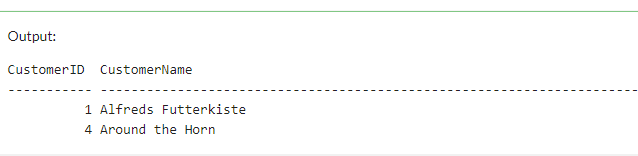
\includegraphics{./Figs/query75.png}
\end{frame}

\begin{frame}[fragile]{Përdorimi i NOT IN}
\phantomsection\label{puxebrdorimi-i-not-in}
Shembull: Të gjithë klientët që nuk janë nga `Germany', `France', ose
`UK':

\begin{Shaded}
\begin{Highlighting}[]
\KeywordTok{SELECT} \OperatorTok{*}
\KeywordTok{FROM}\NormalTok{ Customers}
\KeywordTok{WHERE}\NormalTok{ Country }\KeywordTok{NOT} \KeywordTok{IN}\NormalTok{ (}\StringTok{\textquotesingle{}Germany\textquotesingle{}}\NormalTok{, }\StringTok{\textquotesingle{}France\textquotesingle{}}\NormalTok{, }\StringTok{\textquotesingle{}UK\textquotesingle{}}\NormalTok{);}
\end{Highlighting}
\end{Shaded}
\end{frame}

\begin{frame}[fragile]{Shembull}
\phantomsection\label{shembull-21}
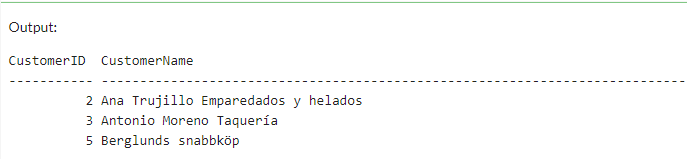
\includegraphics{./Figs/query76.png} \#\# Tabela Orders

\AddToHookNext{env/Highlighting/begin}{\tiny}

\begin{Shaded}
\begin{Highlighting}[]
\CommentTok{{-}{-} Krijo tabelën Orders}
\KeywordTok{CREATE} \KeywordTok{TABLE}\NormalTok{ Orders (}
\NormalTok{    OrderID }\DataTypeTok{int}\NormalTok{,}
\NormalTok{    CustomerID }\DataTypeTok{int}\NormalTok{,}
\NormalTok{    EmployeeID }\DataTypeTok{int}\NormalTok{,}
\NormalTok{    OrderDate }\DataTypeTok{date}\NormalTok{,}
\NormalTok{    ShipperID }\DataTypeTok{int}
\NormalTok{);}
\end{Highlighting}
\end{Shaded}
\end{frame}

\begin{frame}[fragile]{Tabela Orders}
\phantomsection\label{tabela-orders}
\AddToHookNext{env/Highlighting/begin}{\tiny}

\begin{Shaded}
\begin{Highlighting}[]
\CommentTok{{-}{-} Shto të dhënat në tabelën Orders}
\KeywordTok{INSERT} \KeywordTok{INTO}\NormalTok{ Orders (OrderID, CustomerID, EmployeeID, OrderDate, ShipperID) }\KeywordTok{VALUES}
\NormalTok{(}\DecValTok{10248}\NormalTok{, }\DecValTok{1}\NormalTok{, }\DecValTok{5}\NormalTok{, }\StringTok{\textquotesingle{}1996{-}07{-}04\textquotesingle{}}\NormalTok{, }\DecValTok{3}\NormalTok{),}
\NormalTok{(}\DecValTok{10249}\NormalTok{, }\DecValTok{2}\NormalTok{, }\DecValTok{6}\NormalTok{, }\StringTok{\textquotesingle{}1996{-}07{-}05\textquotesingle{}}\NormalTok{, }\DecValTok{1}\NormalTok{),}
\NormalTok{(}\DecValTok{10250}\NormalTok{, }\DecValTok{3}\NormalTok{, }\DecValTok{4}\NormalTok{, }\StringTok{\textquotesingle{}1996{-}07{-}08\textquotesingle{}}\NormalTok{, }\DecValTok{2}\NormalTok{),}
\NormalTok{(}\DecValTok{10251}\NormalTok{, }\DecValTok{4}\NormalTok{, }\DecValTok{3}\NormalTok{, }\StringTok{\textquotesingle{}1996{-}07{-}08\textquotesingle{}}\NormalTok{, }\DecValTok{1}\NormalTok{),}
\NormalTok{(}\DecValTok{10252}\NormalTok{, }\DecValTok{5}\NormalTok{, }\DecValTok{4}\NormalTok{, }\StringTok{\textquotesingle{}1996{-}07{-}09\textquotesingle{}}\NormalTok{, }\DecValTok{2}\NormalTok{);}
\end{Highlighting}
\end{Shaded}
\end{frame}

\begin{frame}[fragile]{Përdorimi i IN me Subquery}
\phantomsection\label{puxebrdorimi-i-in-me-subquery}
Shembull: Të gjithë klientët që kanë një porosi në tabelën Orders:

\begin{Shaded}
\begin{Highlighting}[]
\KeywordTok{SELECT} \OperatorTok{*}
\KeywordTok{FROM}\NormalTok{ Customers}
\KeywordTok{WHERE}\NormalTok{ CustomerID }\KeywordTok{IN}\NormalTok{ (}\KeywordTok{SELECT}\NormalTok{ CustomerID }\KeywordTok{FROM}\NormalTok{ Orders);}
\end{Highlighting}
\end{Shaded}
\end{frame}

\begin{frame}{Shembull}
\phantomsection\label{shembull-22}
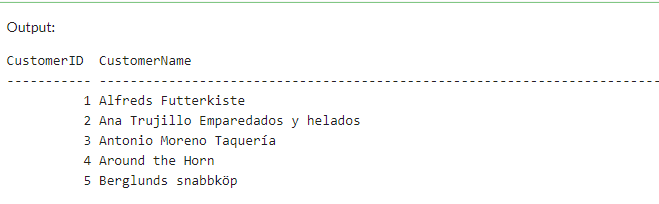
\includegraphics{./Figs/query77.png}
\end{frame}

\begin{frame}[fragile]{Përdorimi i NOT IN me Subquery}
\phantomsection\label{puxebrdorimi-i-not-in-me-subquery}
Shembull: Të gjithë klientët që NUK kanë bërë asnjë porosi në tabelën
Orders:

\begin{Shaded}
\begin{Highlighting}[]
\KeywordTok{SELECT} \OperatorTok{*}
\KeywordTok{FROM}\NormalTok{ Customers}
\KeywordTok{WHERE}\NormalTok{ CustomerID }\KeywordTok{NOT} \KeywordTok{IN}\NormalTok{ (}\KeywordTok{SELECT}\NormalTok{ CustomerID }\KeywordTok{FROM}\NormalTok{ Orders);}
\end{Highlighting}
\end{Shaded}
\end{frame}

\begin{frame}[fragile]{Ushtrime}
\phantomsection\label{ushtrime}
Ushtrim: Përdorni operatorin IN për të zgjedhur të gjitha të dhënat ku
Country është `Norway' ose `France':

\begin{Shaded}
\begin{Highlighting}[]
\KeywordTok{SELECT} \OperatorTok{*}
\KeywordTok{FROM}\NormalTok{ Customers}
\KeywordTok{WHERE}\NormalTok{ Country }\KeywordTok{IN}\NormalTok{ (}\StringTok{\textquotesingle{}Norway\textquotesingle{}}\NormalTok{, }\StringTok{\textquotesingle{}France\textquotesingle{}}\NormalTok{);}
\end{Highlighting}
\end{Shaded}
\end{frame}

\begin{frame}{Funksioni SQL BETWEEN}
\phantomsection\label{funksioni-sql-between}
\begin{itemize}
\item
  Operatori BETWEEN zgjedh vlerat brenda një diapazoni të dhënë.
\item
  Vlerat mund të jenë numra, tekste, ose data.
\item
  Operatori BETWEEN është gjithëpërfshirës: vlerat e fillimit dhe të
  fundit janë të përfshira.
\end{itemize}
\end{frame}

\begin{frame}[fragile]{Sintaksa}
\phantomsection\label{sintaksa-2}
\begin{Shaded}
\begin{Highlighting}[]
\KeywordTok{SELECT}\NormalTok{ kolona\_emri(a)}
\KeywordTok{FROM}\NormalTok{ tabela\_emri}
\KeywordTok{WHERE}\NormalTok{ kolona\_emri }\KeywordTok{BETWEEN}\NormalTok{ vlera1 }\KeywordTok{AND}\NormalTok{ vlera2;}
\end{Highlighting}
\end{Shaded}
\end{frame}

\begin{frame}[fragile]{SQL Query për Krijimin e Tabelës ``Products'' dhe
``Orders'' dhe Shtimin e Të Dhënave}
\phantomsection\label{sql-query-puxebr-krijimin-e-tabeluxebs-products-dhe-orders-dhe-shtimin-e-tuxeb-dhuxebnave}
\begin{Shaded}
\begin{Highlighting}[]
\CommentTok{{-}{-} Krijo tabelën Products}
\KeywordTok{CREATE} \KeywordTok{TABLE}\NormalTok{ Products (}
\NormalTok{    ProductID }\DataTypeTok{int}\NormalTok{,}
\NormalTok{    ProductName }\DataTypeTok{varchar}\NormalTok{(}\DecValTok{255}\NormalTok{),}
\NormalTok{    SupplierID }\DataTypeTok{int}\NormalTok{,}
\NormalTok{    CategoryID }\DataTypeTok{int}\NormalTok{,}
\NormalTok{    Unit }\DataTypeTok{varchar}\NormalTok{(}\DecValTok{255}\NormalTok{),}
\NormalTok{    Price }\DataTypeTok{float}
\NormalTok{);}
\end{Highlighting}
\end{Shaded}
\end{frame}

\begin{frame}[fragile]{SQL Query për Krijimin e Tabelës ``Products'' dhe
``Orders'' dhe Shtimin e Të Dhënave}
\phantomsection\label{sql-query-puxebr-krijimin-e-tabeluxebs-products-dhe-orders-dhe-shtimin-e-tuxeb-dhuxebnave-1}
\AddToHookNext{env/Highlighting/begin}{\tiny}

\begin{Shaded}
\begin{Highlighting}[]
\CommentTok{{-}{-} Shto të dhënat në tabelën Products}
\KeywordTok{INSERT} \KeywordTok{INTO}\NormalTok{ Products (ProductID, ProductName, SupplierID, CategoryID, Unit, Price) }\KeywordTok{VALUES}
\NormalTok{(}\DecValTok{1}\NormalTok{, }\StringTok{\textquotesingle{}Chais\textquotesingle{}}\NormalTok{, }\DecValTok{1}\NormalTok{, }\DecValTok{1}\NormalTok{, }\StringTok{\textquotesingle{}10 boxes x 20 bags\textquotesingle{}}\NormalTok{, }\DecValTok{18}\NormalTok{),}
\NormalTok{(}\DecValTok{2}\NormalTok{, }\StringTok{\textquotesingle{}Chang\textquotesingle{}}\NormalTok{, }\DecValTok{1}\NormalTok{, }\DecValTok{1}\NormalTok{, }\StringTok{\textquotesingle{}24 {-} 12 oz bottles\textquotesingle{}}\NormalTok{, }\DecValTok{19}\NormalTok{),}
\NormalTok{(}\DecValTok{3}\NormalTok{, }\StringTok{\textquotesingle{}Aniseed Syrup\textquotesingle{}}\NormalTok{, }\DecValTok{1}\NormalTok{, }\DecValTok{2}\NormalTok{, }\StringTok{\textquotesingle{}12 {-} 550 ml bottles\textquotesingle{}}\NormalTok{, }\DecValTok{10}\NormalTok{),}
\NormalTok{(}\DecValTok{4}\NormalTok{, }\StringTok{\textquotesingle{}Chef Anton}\CharTok{\textquotesingle{}\textquotesingle{}}\StringTok{s Cajun Seasoning\textquotesingle{}}\NormalTok{, }\DecValTok{2}\NormalTok{, }\DecValTok{2}\NormalTok{, }\StringTok{\textquotesingle{}48 {-} 6 oz jars\textquotesingle{}}\NormalTok{, }\DecValTok{22}\NormalTok{),}
\NormalTok{(}\DecValTok{5}\NormalTok{, }\StringTok{\textquotesingle{}Chef Anton}\CharTok{\textquotesingle{}\textquotesingle{}}\StringTok{s Gumbo Mix\textquotesingle{}}\NormalTok{, }\DecValTok{2}\NormalTok{, }\DecValTok{2}\NormalTok{, }\StringTok{\textquotesingle{}36 boxes\textquotesingle{}}\NormalTok{, }\FloatTok{21.35}\NormalTok{);}
\end{Highlighting}
\end{Shaded}
\end{frame}

\begin{frame}[fragile]{SQL Query për Krijimin e Tabelës ``Products'' dhe
``Orders'' dhe Shtimin e Të Dhënave}
\phantomsection\label{sql-query-puxebr-krijimin-e-tabeluxebs-products-dhe-orders-dhe-shtimin-e-tuxeb-dhuxebnave-2}
\begin{Shaded}
\begin{Highlighting}[]
\CommentTok{{-}{-} Krijo tabelën Orders}
\KeywordTok{CREATE} \KeywordTok{TABLE}\NormalTok{ Orders (}
\NormalTok{    OrderID }\DataTypeTok{int}\NormalTok{,}
\NormalTok{    CustomerID }\DataTypeTok{int}\NormalTok{,}
\NormalTok{    EmployeeID }\DataTypeTok{int}\NormalTok{,}
\NormalTok{    OrderDate }\DataTypeTok{date}\NormalTok{,}
\NormalTok{    ShipperID }\DataTypeTok{int}
\NormalTok{);}
\end{Highlighting}
\end{Shaded}
\end{frame}

\begin{frame}[fragile]{SQL Query për Krijimin e Tabelës ``Products'' dhe
``Orders'' dhe Shtimin e Të Dhënave}
\phantomsection\label{sql-query-puxebr-krijimin-e-tabeluxebs-products-dhe-orders-dhe-shtimin-e-tuxeb-dhuxebnave-3}
\AddToHookNext{env/Highlighting/begin}{\tiny}

\begin{Shaded}
\begin{Highlighting}[]

\CommentTok{{-}{-} Shto të dhënat në tabelën Orders}
\KeywordTok{INSERT} \KeywordTok{INTO}\NormalTok{ Orders (OrderID, CustomerID, EmployeeID, OrderDate, ShipperID) }\KeywordTok{VALUES}
\NormalTok{(}\DecValTok{10248}\NormalTok{, }\DecValTok{1}\NormalTok{, }\DecValTok{5}\NormalTok{, }\StringTok{\textquotesingle{}1996{-}07{-}04\textquotesingle{}}\NormalTok{, }\DecValTok{3}\NormalTok{),}
\NormalTok{(}\DecValTok{10249}\NormalTok{, }\DecValTok{2}\NormalTok{, }\DecValTok{6}\NormalTok{, }\StringTok{\textquotesingle{}1996{-}07{-}05\textquotesingle{}}\NormalTok{, }\DecValTok{1}\NormalTok{),}
\NormalTok{(}\DecValTok{10250}\NormalTok{, }\DecValTok{3}\NormalTok{, }\DecValTok{4}\NormalTok{, }\StringTok{\textquotesingle{}1996{-}07{-}08\textquotesingle{}}\NormalTok{, }\DecValTok{2}\NormalTok{),}
\NormalTok{(}\DecValTok{10251}\NormalTok{, }\DecValTok{4}\NormalTok{, }\DecValTok{3}\NormalTok{, }\StringTok{\textquotesingle{}1996{-}07{-}08\textquotesingle{}}\NormalTok{, }\DecValTok{1}\NormalTok{),}
\NormalTok{(}\DecValTok{10252}\NormalTok{, }\DecValTok{5}\NormalTok{, }\DecValTok{4}\NormalTok{, }\StringTok{\textquotesingle{}1996{-}07{-}09\textquotesingle{}}\NormalTok{, }\DecValTok{2}\NormalTok{);}
\end{Highlighting}
\end{Shaded}
\end{frame}

\begin{frame}[fragile]{Përdorimi i BETWEEN për Numra}
\phantomsection\label{puxebrdorimi-i-between-puxebr-numra}
Shembull: Zgjedh të gjitha produktet me çmim midis 10 dhe 20:

\begin{Shaded}
\begin{Highlighting}[]
\KeywordTok{SELECT} \OperatorTok{*}
\KeywordTok{FROM}\NormalTok{ Products}
\KeywordTok{WHERE}\NormalTok{ Price }\KeywordTok{BETWEEN} \DecValTok{10} \KeywordTok{AND} \DecValTok{20}\NormalTok{;}
\end{Highlighting}
\end{Shaded}
\end{frame}

\begin{frame}{Shembull}
\phantomsection\label{shembull-23}
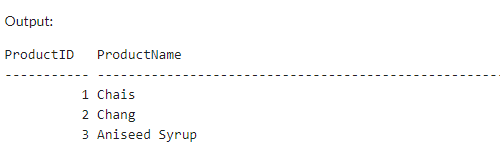
\includegraphics{./Figs/query78.png}
\end{frame}

\begin{frame}[fragile]{Përdorimi i NOT BETWEEN për Numra}
\phantomsection\label{puxebrdorimi-i-not-between-puxebr-numra}
Shembull: Zgjedh të gjitha produktet jashtë diapazonit 10 dhe 20:

\begin{Shaded}
\begin{Highlighting}[]
\KeywordTok{SELECT} \OperatorTok{*}
\KeywordTok{FROM}\NormalTok{ Products}
\KeywordTok{WHERE}\NormalTok{ Price }\KeywordTok{NOT} \KeywordTok{BETWEEN} \DecValTok{10} \KeywordTok{AND} \DecValTok{20}\NormalTok{;}
\end{Highlighting}
\end{Shaded}
\end{frame}

\begin{frame}{Shembull}
\phantomsection\label{shembull-24}
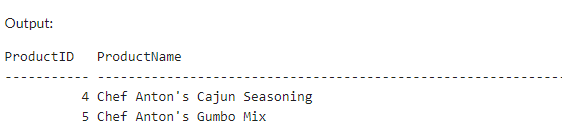
\includegraphics{./Figs/query79.png}
\end{frame}

\begin{frame}[fragile]{Përdorimi i BETWEEN me IN}
\phantomsection\label{puxebrdorimi-i-between-me-in}
Shembull: Zgjedh të gjitha produktet me çmim midis 10 dhe 20 dhe
CategoryID të jetë 1, 2 ose 3:

\begin{Shaded}
\begin{Highlighting}[]
\KeywordTok{SELECT} \OperatorTok{*}
\KeywordTok{FROM}\NormalTok{ Products}
\KeywordTok{WHERE}\NormalTok{ Price }\KeywordTok{BETWEEN} \DecValTok{10} \KeywordTok{AND} \DecValTok{20}
\KeywordTok{AND}\NormalTok{ CategoryID }\KeywordTok{IN}\NormalTok{ (}\DecValTok{1}\NormalTok{, }\DecValTok{2}\NormalTok{, }\DecValTok{3}\NormalTok{);}
\end{Highlighting}
\end{Shaded}
\end{frame}

\begin{frame}{Shembull}
\phantomsection\label{shembull-25}
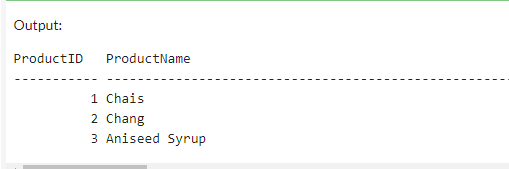
\includegraphics{./Figs/query80.png}
\end{frame}

\begin{frame}[fragile]{Përdorimi i BETWEEN për Tekste}
\phantomsection\label{puxebrdorimi-i-between-puxebr-tekste}
Shembull: Zgjedh të gjitha produktet me emër alfabetikisht midis
`Carnarvon Tigers' dhe `Mozzarella di Giovanni':

\AddToHookNext{env/Highlighting/begin}{\tiny}

\begin{Shaded}
\begin{Highlighting}[]
\KeywordTok{SELECT} \OperatorTok{*}
\KeywordTok{FROM}\NormalTok{ Products}
\KeywordTok{WHERE}\NormalTok{ ProductName }\KeywordTok{BETWEEN} \StringTok{\textquotesingle{}Carnarvon Tigers\textquotesingle{}} \KeywordTok{AND} \StringTok{\textquotesingle{}Mozzarella di Giovanni\textquotesingle{}}
\KeywordTok{ORDER} \KeywordTok{BY}\NormalTok{ ProductName;}
\end{Highlighting}
\end{Shaded}
\end{frame}

\begin{frame}{Shembull}
\phantomsection\label{shembull-26}
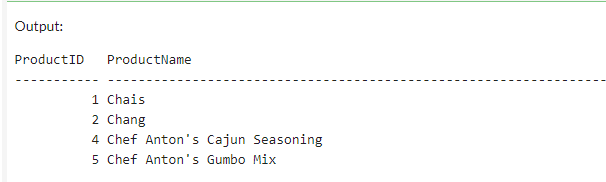
\includegraphics{./Figs/query81.png}
\end{frame}

\begin{frame}[fragile]{Përdorimi i NOT BETWEEN për Tekste}
\phantomsection\label{puxebrdorimi-i-not-between-puxebr-tekste}
Shembull: Zgjedh të gjitha produktet me emër që nuk janë midis
`Carnarvon Tigers' dhe `Mozzarella di Giovanni':

\AddToHookNext{env/Highlighting/begin}{\tiny}

\begin{Shaded}
\begin{Highlighting}[]
\KeywordTok{SELECT} \OperatorTok{*}
\KeywordTok{FROM}\NormalTok{ Products}
\KeywordTok{WHERE}\NormalTok{ ProductName }\KeywordTok{NOT} \KeywordTok{BETWEEN} \StringTok{\textquotesingle{}Carnarvon Tigers\textquotesingle{}} \KeywordTok{AND} \StringTok{\textquotesingle{}Mozzarella di Giovanni\textquotesingle{}}
\KeywordTok{ORDER} \KeywordTok{BY}\NormalTok{ ProductName;}
\end{Highlighting}
\end{Shaded}
\end{frame}

\begin{frame}{Shembull}
\phantomsection\label{shembull-27}
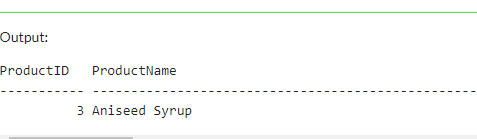
\includegraphics{./Figs/query82.png}
\end{frame}

\begin{frame}[fragile]{Përdorimi i BETWEEN për Data}
\phantomsection\label{puxebrdorimi-i-between-puxebr-data}
Shembull: Zgjedh të gjitha porositë me datë porosie midis
`01-Korrik-1996' dhe `31-Korrik-1996':

\AddToHookNext{env/Highlighting/begin}{\tiny}

\begin{Shaded}
\begin{Highlighting}[]
\KeywordTok{SELECT} \OperatorTok{*}
\KeywordTok{FROM}\NormalTok{ Orders}
\KeywordTok{WHERE}\NormalTok{ OrderDate }\KeywordTok{BETWEEN} \StringTok{\textquotesingle{}1996{-}07{-}01\textquotesingle{}} \KeywordTok{AND} \StringTok{\textquotesingle{}1996{-}07{-}31\textquotesingle{}}\NormalTok{;}
\end{Highlighting}
\end{Shaded}
\end{frame}

\begin{frame}{Shembull}
\phantomsection\label{shembull-28}
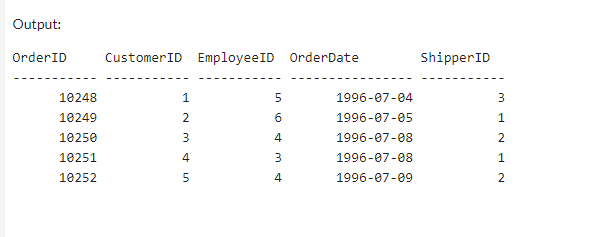
\includegraphics{./Figs/query83.png}
\end{frame}

\begin{frame}[fragile]{Ushtrim: Përdorni operatorin BETWEEN për të
zgjedhur të gjitha të dhënat ku vlera e kolonës Price është midis 10 dhe
20:}
\phantomsection\label{ushtrim-puxebrdorni-operatorin-between-puxebr-tuxeb-zgjedhur-tuxeb-gjitha-tuxeb-dhuxebnat-ku-vlera-e-kolonuxebs-price-uxebshtuxeb-midis-10-dhe-20}
\AddToHookNext{env/Highlighting/begin}{\tiny}

\begin{Shaded}
\begin{Highlighting}[]
\KeywordTok{SELECT} \OperatorTok{*}
\KeywordTok{FROM}\NormalTok{ Products}
\KeywordTok{WHERE}\NormalTok{ Price }\KeywordTok{BETWEEN} \DecValTok{10} \KeywordTok{AND} \DecValTok{20}\NormalTok{;}
\end{Highlighting}
\end{Shaded}
\end{frame}

\begin{frame}{SQL JOIN}
\phantomsection\label{sql-join}
Një klauzolë JOIN përdoret për të kombinuar rreshtat nga dy ose më shumë
tabela, bazuar në një kolonë të lidhur midis tyre.
\end{frame}

\begin{frame}[fragile]{Sintaksa}
\phantomsection\label{sintaksa-3}
\AddToHookNext{env/Highlighting/begin}{\tiny}

\begin{Shaded}
\begin{Highlighting}[]
\KeywordTok{SELECT}\NormalTok{ kolona\_emri(a)}
\KeywordTok{FROM}\NormalTok{ tabela1}
\KeywordTok{JOIN}\NormalTok{ tipi\_i\_join}
\KeywordTok{ON}\NormalTok{ tabela1.kolona\_e\_lidhur }\OperatorTok{=}\NormalTok{ tabela2.kolona\_e\_lidhur;}
\end{Highlighting}
\end{Shaded}
\end{frame}

\begin{frame}[fragile]{SQL Query për Krijimin e Tabelave ``Customers''
dhe ``Orders'' dhe Shtimin e Të Dhënave}
\phantomsection\label{sql-query-puxebr-krijimin-e-tabelave-customers-dhe-orders-dhe-shtimin-e-tuxeb-dhuxebnave}
\AddToHookNext{env/Highlighting/begin}{\tiny}

\begin{Shaded}
\begin{Highlighting}[]

\CommentTok{{-}{-} Krijo tabelën Customers}
\KeywordTok{CREATE} \KeywordTok{TABLE}\NormalTok{ Customers (}
\NormalTok{    CustomerID }\DataTypeTok{int}\NormalTok{,}
\NormalTok{    CustomerName }\DataTypeTok{varchar}\NormalTok{(}\DecValTok{255}\NormalTok{),}
\NormalTok{    ContactName }\DataTypeTok{varchar}\NormalTok{(}\DecValTok{255}\NormalTok{),}
\NormalTok{    Country }\DataTypeTok{varchar}\NormalTok{(}\DecValTok{100}\NormalTok{)}
\NormalTok{);}
\end{Highlighting}
\end{Shaded}
\end{frame}

\begin{frame}[fragile]{SQL Query për Krijimin e Tabelave ``Customers''
dhe ``Orders'' dhe Shtimin e Të Dhënave}
\phantomsection\label{sql-query-puxebr-krijimin-e-tabelave-customers-dhe-orders-dhe-shtimin-e-tuxeb-dhuxebnave-1}
\AddToHookNext{env/Highlighting/begin}{\tiny}

\begin{Shaded}
\begin{Highlighting}[]

\CommentTok{{-}{-} Shto të dhënat në tabelën Customers}
\KeywordTok{INSERT} \KeywordTok{INTO}\NormalTok{ Customers (CustomerID, CustomerName, ContactName, Country) }\KeywordTok{VALUES}
\NormalTok{(}\DecValTok{1}\NormalTok{, }\StringTok{\textquotesingle{}Alfreds Futterkiste\textquotesingle{}}\NormalTok{, }\StringTok{\textquotesingle{}Maria Anders\textquotesingle{}}\NormalTok{, }\StringTok{\textquotesingle{}Germany\textquotesingle{}}\NormalTok{),}
\NormalTok{(}\DecValTok{2}\NormalTok{, }\StringTok{\textquotesingle{}Ana Trujillo Emparedados y helados\textquotesingle{}}\NormalTok{, }\StringTok{\textquotesingle{}Ana Trujillo\textquotesingle{}}\NormalTok{, }\StringTok{\textquotesingle{}Mexico\textquotesingle{}}\NormalTok{),}
\NormalTok{(}\DecValTok{3}\NormalTok{, }\StringTok{\textquotesingle{}Antonio Moreno Taquería\textquotesingle{}}\NormalTok{, }\StringTok{\textquotesingle{}Antonio Moreno\textquotesingle{}}\NormalTok{, }\StringTok{\textquotesingle{}Mexico\textquotesingle{}}\NormalTok{);}
\end{Highlighting}
\end{Shaded}
\end{frame}

\begin{frame}[fragile]{SQL Query për Krijimin e Tabelave ``Customers''
dhe ``Orders'' dhe Shtimin e Të Dhënave}
\phantomsection\label{sql-query-puxebr-krijimin-e-tabelave-customers-dhe-orders-dhe-shtimin-e-tuxeb-dhuxebnave-2}
\AddToHookNext{env/Highlighting/begin}{\tiny}

\begin{Shaded}
\begin{Highlighting}[]

\CommentTok{{-}{-} Krijo tabelën Orders}
\KeywordTok{CREATE} \KeywordTok{TABLE}\NormalTok{ Orders (}
\NormalTok{    OrderID }\DataTypeTok{int}\NormalTok{,}
\NormalTok{    CustomerID }\DataTypeTok{int}\NormalTok{,}
\NormalTok{    OrderDate }\DataTypeTok{date}
\NormalTok{);}
\end{Highlighting}
\end{Shaded}
\end{frame}

\begin{frame}[fragile]{SQL Query për Krijimin e Tabelave ``Customers''
dhe ``Orders'' dhe Shtimin e Të Dhënave}
\phantomsection\label{sql-query-puxebr-krijimin-e-tabelave-customers-dhe-orders-dhe-shtimin-e-tuxeb-dhuxebnave-3}
\AddToHookNext{env/Highlighting/begin}{\tiny}

\begin{Shaded}
\begin{Highlighting}[]
\CommentTok{{-}{-} Shto të dhënat në tabelën Orders}
\KeywordTok{INSERT} \KeywordTok{INTO}\NormalTok{ Orders (OrderID, CustomerID, OrderDate) }\KeywordTok{VALUES}
\NormalTok{(}\DecValTok{10308}\NormalTok{, }\DecValTok{2}\NormalTok{, }\StringTok{\textquotesingle{}1996{-}09{-}18\textquotesingle{}}\NormalTok{),}
\NormalTok{(}\DecValTok{10309}\NormalTok{, }\DecValTok{37}\NormalTok{, }\StringTok{\textquotesingle{}1996{-}09{-}19\textquotesingle{}}\NormalTok{),}
\NormalTok{(}\DecValTok{10310}\NormalTok{, }\DecValTok{77}\NormalTok{, }\StringTok{\textquotesingle{}1996{-}09{-}20\textquotesingle{}}\NormalTok{);}
\end{Highlighting}
\end{Shaded}
\end{frame}

\begin{frame}[fragile]{Shembull: INNER JOIN}
\phantomsection\label{shembull-inner-join}
Shembull: Zgjedh rreshtat që kanë vlera të përshtatshme në të dyja
tabelat:

\AddToHookNext{env/Highlighting/begin}{\tiny}

\begin{Shaded}
\begin{Highlighting}[]

\KeywordTok{SELECT}\NormalTok{ Orders.OrderID, Customers.CustomerName, Orders.OrderDate}
\KeywordTok{FROM}\NormalTok{ Orders}
\KeywordTok{INNER} \KeywordTok{JOIN}\NormalTok{ Customers }\KeywordTok{ON}\NormalTok{ Orders.CustomerID}\OperatorTok{=}\NormalTok{Customers.CustomerID;}
\end{Highlighting}
\end{Shaded}
\end{frame}

\begin{frame}{Shembull}
\phantomsection\label{shembull-29}
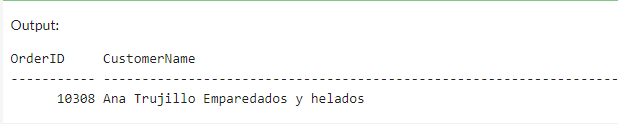
\includegraphics{./Figs/query84.png}
\end{frame}

\begin{frame}{Llojet e Ndryshme të JOINs në SQL}
\phantomsection\label{llojet-e-ndryshme-tuxeb-joins-nuxeb-sql}
\begin{itemize}
\item
  INNER JOIN: Kthen rreshtat që kanë vlera të përshtatshme në të dyja
  tabelat.
\item
  LEFT (OUTER) JOIN: Kthen të gjithë rreshtat nga tabela e majtë dhe
  rreshtat e përshtatshme nga tabela e djathtë.
\item
  RIGHT (OUTER) JOIN: Kthen të gjithë rreshtat nga tabela e djathtë dhe
  rreshtat e përshtatshme nga tabela e majtë.
\item
  FULL (OUTER) JOIN: Kthen të gjithë rreshtat kur ka një përputhje në
  secilën nga tabelat e majta ose të djathta.
\end{itemize}
\end{frame}

\begin{frame}[fragile]{Përdorimi i LEFT JOIN}
\phantomsection\label{puxebrdorimi-i-left-join}
Shembull: Zgjedh të gjithë rreshtat nga tabela e majtë dhe rreshtat e
përshtatshme nga tabela e djathtë:

\AddToHookNext{env/Highlighting/begin}{\tiny}

\begin{Shaded}
\begin{Highlighting}[]
\KeywordTok{SELECT}\NormalTok{ Orders.OrderID, Customers.CustomerName, Orders.OrderDate}
\KeywordTok{FROM}\NormalTok{ Orders}
\KeywordTok{LEFT} \KeywordTok{JOIN}\NormalTok{ Customers }\KeywordTok{ON}\NormalTok{ Orders.CustomerID}\OperatorTok{=}\NormalTok{Customers.CustomerID;}
\end{Highlighting}
\end{Shaded}
\end{frame}

\begin{frame}{Shembull}
\phantomsection\label{shembull-30}
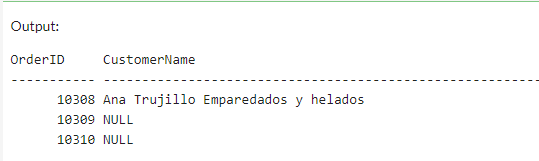
\includegraphics{./Figs/query85.png}
\end{frame}

\begin{frame}[fragile]{Përdorimi i RIGHT JOIN}
\phantomsection\label{puxebrdorimi-i-right-join}
Shembull: Zgjedh të gjithë rreshtat nga tabela e djathtë dhe rreshtat e
përshtatshme nga tabela e majtë:

\AddToHookNext{env/Highlighting/begin}{\tiny}

\begin{Shaded}
\begin{Highlighting}[]
\KeywordTok{SELECT}\NormalTok{ Orders.OrderID, Customers.CustomerName, Orders.OrderDate}
\KeywordTok{FROM}\NormalTok{ Orders}
\KeywordTok{RIGHT} \KeywordTok{JOIN}\NormalTok{ Customers }\KeywordTok{ON}\NormalTok{ Orders.CustomerID}\OperatorTok{=}\NormalTok{Customers.CustomerID;}
\end{Highlighting}
\end{Shaded}
\end{frame}

\begin{frame}{Shembull}
\phantomsection\label{shembull-31}
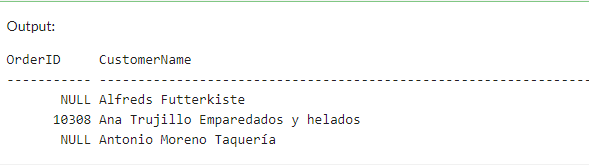
\includegraphics{./Figs/query86.png}
\end{frame}

\begin{frame}[fragile]{Përdorimi i FULL OUTER JOIN}
\phantomsection\label{puxebrdorimi-i-full-outer-join}
Shembull: Zgjedh të gjithë rreshtat kur ka një përputhje në secilën nga
tabelat e majta ose të djathta:

\AddToHookNext{env/Highlighting/begin}{\tiny}

\begin{Shaded}
\begin{Highlighting}[]
\KeywordTok{SELECT}\NormalTok{ Orders.OrderID, Customers.CustomerName, Orders.OrderDate}
\KeywordTok{FROM}\NormalTok{ Orders}
\KeywordTok{FULL} \KeywordTok{OUTER} \KeywordTok{JOIN}\NormalTok{ Customers }\KeywordTok{ON}\NormalTok{ Orders.CustomerID}\OperatorTok{=}\NormalTok{Customers.CustomerID;}
\end{Highlighting}
\end{Shaded}
\end{frame}

\begin{frame}{Shembull}
\phantomsection\label{shembull-32}
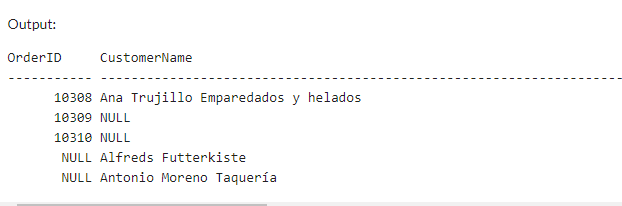
\includegraphics{./Figs/query87.png}
\end{frame}

\begin{frame}[fragile]{Ushtrim}
\phantomsection\label{ushtrim}
Ushtrim: Përmbushni pjesët e mungesë në klauzolën JOIN për të bashkuar
tabelat Orders dhe Customers, duke përdorur fushën CustomerID si lidhje
midis të dyjave:

\AddToHookNext{env/Highlighting/begin}{\tiny}

\begin{Shaded}
\begin{Highlighting}[]
\KeywordTok{SELECT} \OperatorTok{*}
\KeywordTok{FROM}\NormalTok{ Orders}
\KeywordTok{LEFT} \KeywordTok{JOIN}\NormalTok{ Customers}
\KeywordTok{ON}\NormalTok{ Orders.CustomerID }\OperatorTok{=}\NormalTok{ Customers.CustomerID;}
\end{Highlighting}
\end{Shaded}
\end{frame}

\end{document}
